%% The following is a directive for TeXShop to indicate the main file
%%!TEX root = main.tex

% ===========================================================================================
\chapter{\textbf{Approach}}
\label{sec3:Approach}

In this chapter, the approach taken to build the generic IDS is discussed.
Firstly, the threat model is presented, followed by an introduction to HMMs which are employed to find the correlation between the logical properties of the system to detect intrusions. Secondly, the work-flow of CORGIDS and an example to illustrate the work-flow are detailed in this chapter. 

\section{Threat Model}
\label{sec:threatModel}
{\bf Access}: The term System Under Test (SUT) in this study is used to represent the system on which the analysis is performed. It is assumed that the attacker has the capability to gain read and write access to the communication channel between the SUT and the controller. Using this access, the attacker can modify the contents or add data packets being transferred. This assumption is realistic as previous work~\cite{ericsson2010cyber} has shown that such access is rather easy to get.

Further, it is assumed that the attacker has the \textit{root} access to the SUT, which means that the application code can be modified to suit the attacker's needs. However, as an attacker is likely to want to remain stealthy, it is more likely to make small changes to the program rather than large-scale changes such as replacing the entire program with their own. Also, an assumption that the attacker cannot modify the operating system kernel or the device firmware is made. This can be ensured by using code signing or trusted computing hardware if it is available. 

{\bf Capabilities}: It is assumed that the attacker, using access to the communication channel, can perform two types of attacks. The first one is spoofing, where the contents of the data packets can be modified, and the second one is flooding where the number of data packets being sent to the controller can be increased. The attacker can also perform physical attacks on the CPS, for example by rebooting it, at arbitrary points in time. 
 
For this research, attacks such as network attacks such as Denial-of-Service (DoS) or message dropping attacks are \textit{not} considered . Also, only attacks that change the correlation between the logical properties are considered. Therefore, attacks which do not create an impact on the logical properties are not considered. 

\section{Hidden Markov Models}
\label{sec:HMM_explain}

In this study, an IDS is built which internally uses an HMM to find logical correlations among the physical variables in a system. HMMs are useful for systems which can be represented by sequences or time series. An HMM is a finite model that can be used to describe a probability distribution over an infinite number of possible sequences in a given system~\cite{eddy1996hidden}.

Unlike a simple Markov model, an HMM is composed of a number of hidden states. Each hidden state 'emits' symbols according to emission probabilities, and the states are interconnected by state-transition probabilities. Starting from an initial state, a sequence of states is generated by moving from state to state according to the state-transition probabilities until an end state is reached. Each state then emits symbols according to that state's emission probability distribution, creating an observable sequence of symbols.
More formally, an HMM can be represented by ( $\pi$, A, $\theta$) where $\pi$ represents the starting probability of the transitions between the hidden states, while the transition probability matrix is denoted by A and $\theta$ represents the emission probability of the hidden states.

HMMs are a good fit for problems in which i) the model parameters and observed data are present, and there is a need to estimate the sequence of hidden states; ii) the observed data is given and the model parameters are to be estimated, and iii) the information of model parameters and observed data is present while there is a need to find the likelihood of the data. In CORGIDS, HMMs are used for the third kind of problem, i.e., the likelihood of the current observed data belonging to the predefined model's parameters is measured. In order to do so, the values of correlated physical properties of the system are fed into an HMM, which then infers the correlations between them. These correlations are then used to determine the likelihood of the current observed data as stemming from the model and its parameters. Any deviation is signaled as an anomaly and a possible security attack.

HMMs act as the core of intrusion detection module mainly because they are capable of finding data patterns in high dimensional, non-linear time series based data systems. Also, HMMs work by creating hidden states and then transitioning between them which is very similar to the operations of CPS system, which are typically modeled as state machines.
Unlike techniques such as correlation coefficients, HMMs are also highly resilient to noise and outliers. 
For instance, Krotofil et al.~\cite{krotofil2015process} use Pearson Correlation Coefficient(PCC) to determine correlation for the cluster entropy. PCC measures linear correlation among the variables, therefore is not suitable for multidimensional non-linear data. Also the variables undergoing PCC must be either based on interval or ratio scale, making this approach much less generic. Chen at el.  \cite{chen2018learning} employ SVMs to detect an anomaly in a time series based system. Unfortunately, SVMs do not work well with time series data, because they work with a snapshot of the state and classify it into a class. However, by manipulating the input feature vector to the SVM in such a way that it encapsulates the time factor, authors use it for anomaly detection. On the other hand, Aliabadi et al. ~\cite{aliabadi2017artinali} use Frequent Item Set Mining algorithm which does not model the system, but mines the data under different events. Unfortunately, they do not consider the physical properties, except time, of the CPS. Iturbe et al. \cite{iturbe2017feasibility} use Principal Component Analysis (PCA) which infers correlation among the variables and is better suited for linear correlations, as it works by generating orthogonal projections. However, for non-linearly correlated data as in our case, PCA is not able to find correlations.

\section{Work-flow of CORGIDS}
CORGIDS is a generic intrusion detection system which exploits the correlation of the logical properties of the SUT to detect intrusions. ~\autoref{fig:workflow} shows the key components and the work flow of CORGIDS.

\begin{figure}[ht]
    \centering
    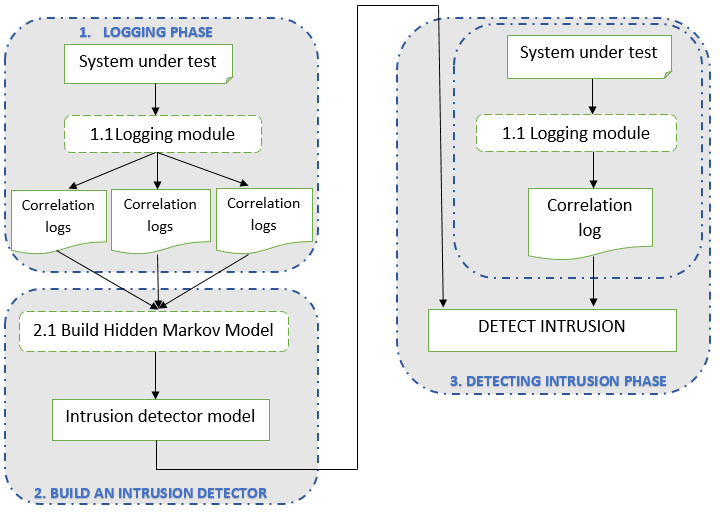
\includegraphics[scale=0.50,keepaspectratio = true]{Graphics/CORGIDSWorkflowNew.png}
    \caption{Workflow of CORGIDS}
    \label{fig:workflow}
\end{figure}

CORGIDS workflow can be broken down into three main phases, namely, a) Logging Phase; b) Building an Intrusion Detector Phase; and c) Detecting Intrusion Phase. Each of the phases are explained below.

\begin{enumerate}
\item {Logging Phase}: The \textit{1. Logging Phase} in ~\autoref{fig:workflow} is the starting point for building an intrusion detector and for deploying it on a system for which intrusion detection is desired. SUT is an input to this phase and is passed through the \textit{1.1 Logging module} in which it is manually instrumented to collect the values of the correlated properties\footnote{The approach of manually instrumenting the code to collect logs has been used by prior work~\cite{chen2018learning,aliabadi2017artinali}}. These properties are chosen by the user of the intrusion detection system based on the general knowledge of the SUT. This phase will ensure that the traces which contain the values of the properties while the system is running are collected. Also, it is assumed that the source code of the SUT is available and can be modified for instrumentation - this is reasonable as the developer of the system will deploy CORGIDS. At the end of this \textit{logging phase}, the system traces containing the values of the logical properties of the SUT are collected.

\item {Building an Intrusion Detector}: In this phase, the system traces collected from the \textit{Logging Phase} are used to build an HMM which behaviorally represents the SUT. The pseudo code of the algorithm for building an intrusion detector is described below. To build an intrusion detector the system traces are fed into the HMM model for its training in Line 2.

\begin{comment}
\makeatletter
\renewcommand{\fnum@algorithm}{\fname@algorithm}
\def\BState{\State\hskip-\ALG@thistlm}
\makeatother
\end{comment}

\begin{comment}
\begin{algorithm}
\caption{Building an intrusion detector}
\begin{algorithmic}
\Procedure{BuildAnIntrusionDetector }{\textit{logs}}\text{:}
\State $\textit{trainedModel} = \text{trainHMMModel (\textit{logs})}$
\item for \textit{l} in logs
\State $\textit{logLikelihood(i)} = log(\textit{trainedModel(l)})$
\State $\text{\textit{S}} = \text{sum of all \textit{logLikelihood(i)'s}}$
\item $\textit{M} = \text{mean of \textit{S}}$
\item \textbf{return \textit{trainedModel}, \textit{M}};
\EndProcedure

\Procedure{trainHMMModel }{\textit{logs}}\text{:}
\item for $hiddenStates = 2$, $hiddenStates {+}{+}$
\State \textbf{create an HMM model} \textit{model}(i);
\State $\textit{logLikelihood(i)} = \text{log(\textit{model}(i))}$
\If {$\delta$$\text{ (\textit{logLikelihood})} < \textit{Threshold}$}
\State \textbf{return \textit{model}(i)};
\EndIf
\EndProcedure
\end{algorithmic}
\end{algorithm}
\end{comment}

\begin{figure}[ht]
    \centering
    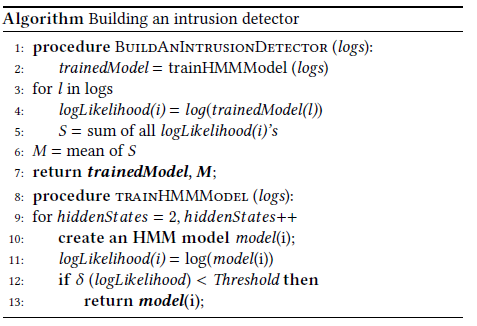
\includegraphics[scale=0.75,keepaspectratio = true]{Graphics/Algo.png}
    \label{fig:algo}
\end{figure}

Training of an HMM is begun in \textit{procedure TRAINHMMMODEL} in Line 8, by varying the number of \textit{hiddenStates}. The number of hidden states is a free parameter of an HMM which needs tuning in order to create a model which can be used for intrusion detection. Iteration begins with HMM's \textit{model(i)} with the starting value of two hidden states and is kept on increasing by one (Line 9 - 10). The log likelihood of the \textit{model(i)} is calculated which represents the goodness of the \textit{model(i)} fit of the model to the data that was used for constructing it.
The log likelihood is stored in variable \textit{logLikelihood(i)} as shown in Line 11. The \textit{threshold} in Line 12 represents the minimum difference between the current and previous HMM's log likelihood. Using threshold as a stopping criteria for HMM has also been used in prior work~\cite{ferrer2000influence}. The best HMM is returned in Line 13  with its parameters as the model to be used for intrusion detection. At this point the \textit{trainedHMMModel} is used to calculate the log likelihood for each of the training system traces (Line 3). As a by product, the mean of log likelihood is calculated (Line 5- 6) to get the estimated log likelihood value \textit{M} (Line 6) for a training log. \textit{M} is then used for comparison in the later steps to detect intrusion. Creating HMMs by increasing the number of hidden states uses a significant amount of memory and computational power.
However as this phase needs to be carried out just once for a SUT, it is not a major bottleneck. Once the intrusion detector HMM is created, it can be used to detect an anomaly in the next phase. 

\item {Detecting Intrusion Phase}: This phase starts with the \textit{Logging Phase} which is used to collect the system trace from the SUT while it is running. In this phase, only the system trace corresponding to the running SUT is collected, rather than many different system traces. 
The trace generated is then used together with the intrusion detector built in the \textit{Building an Intrusion Detector Phase}. Using the HMM model and its saved parameters, the log likelihood of the current system trace is calculated and compared with the mean log likelihood \textit{M} calculated in the \textit{Building an Intrusion Detector} in Line 6. If the log likelihood of the system trace is less than a specified range ($\delta$) from \textit{M}, it signifies that the system trace does not follow the behavior which was observed when the HMM was being trained. 
The specified range ($\delta$) is found by running a sensitivity analysis (Section \ref{sensitivityAnalysis}). Further, as the system traces used for building the HMM were assumed to be correct (i.e., not attacked), this implies that the current system trace represents a system under attack.  
Thus, current state of the SUT is flagged to be malicious. 
\end{enumerate}


\section{Example}

\begin{figure}[ht]
    \centering
    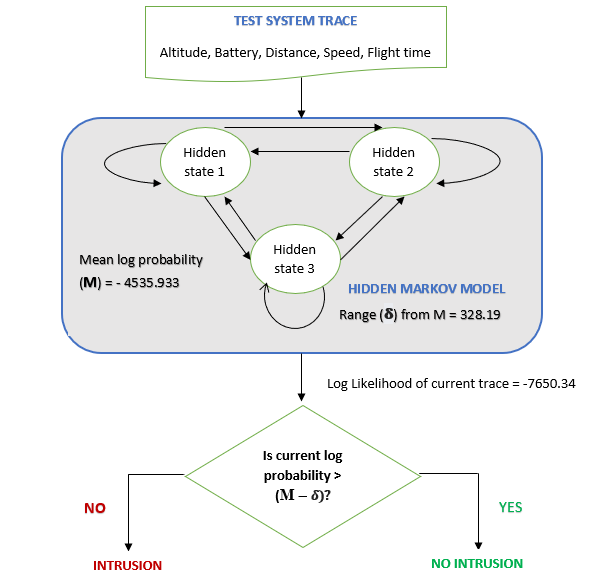
\includegraphics[scale=0.55,keepaspectratio = true]{Graphics/CORGIDSApproach.png}
    \caption{Approach of CORGIDS}
    \label{fig:approach}
\end{figure}

The earlier example of an UAV from chapter \ref{ch:Introduction} is used in this section to illustrate how CORGIDS can be used to detect intrusions in ~\autoref{fig:approach}. As described in chapter \ref{ch:Introduction}, an UAV has physical properties such as the current altitude, battery percentage left, distance traveled, current speed and flight time. These physical properties are correlated to each other as per the laws of physics. Here, the approach which will detect an intrusion in an UAV is elaborated, using the work-flow described in \ref{fig:approach}. Distance spoofing scenario of the UAV is used as an example.

First the \textit{Logging Phase} starts, where the UAV is instrumented to collect the correlated properties such as current altitude, current battery percentage left, distance traveled, current speed and flight time. The above properties are collected at regular intervals of time to form the system traces. A section of the sample system trace collected is shown in Table~\ref{tab:nonFaultyCorrelationLog}. In the trace, it can be observed that all the properties are correlated  with each other, and that the correlations are fairly stable. For instance, if the \textit{Speed} of the UAV increases, the \textit{Distance traveled} will also increase. Further, the \textit{Distance traveled} property can have values that are either increasing or stagnant. Multiple iterations of the UAV were run by varying the routes it travels, to collect non-faulty system traces from it.

\begin{table}
\centering
  \caption{Slice of a non-faulty system trace obtained while flying an UAV on a random route}
  \label{tab:nonFaultyCorrelationLog}
  \scalebox{0.9}{
  \begin{tabular}{|p{1.2cm}|p{1cm}|p{1.85cm}|p{0.9cm}|p{1.7cm}|}
 \toprule
\textbf{Altitude (m)}&\textbf{Battery left (\%)}&\textbf{Distance travelled (m)}&\textbf{Speed (m/s)}&\textbf{Flight time (s)}\\
  \hline
..&..&..&..&..\\
40&89&42.1445&1&38.32\\
40&89&44.2563&2&39.342\\
40	&89	&47.2397	&3	&40.356\\
40	&89	&51.0202	&3	&41.376\\
40	&88	&55.2434	&4	&42.345\\
40	&88	&59.5897	&4	&43.346\\
40	&88	&64.1632	&4	&44.335\\
41	&88	&68.8979	&4	&45.323\\
41	&88	&73.7389	&4	&46.351\\
41	&87	&78.6564	&4	&47.448\\
41	&87	&83.6196	&4	&48.551\\
41	&87	&88.6138	&4	&49.61\\
41	&87	&93.627	    &5	&50.604\\
41	&86	&98.6659	&5	&51.507\\
..&..&..&..&..\\
\hline
\end{tabular}
}
\end{table}

\begin{table}
\centering
\caption{Slice of a faulty system trace obtained while an UAV was flying on a random route and infected by distance spoofing attack}
\label{tab:faultyCorrelationLog}
\scalebox{0.9}{
\begin{tabular}{|p{1.2cm}|p{1cm}|p{1.85cm}|p{0.9cm}|p{1.7cm}|}
\toprule   \textbf{Altitude (m)}&\textbf{Battery left (\%)}&\textbf{Distance traveled (m)}&\textbf{Speed (m/s)}&\textbf{Flight time (s)}\\
  \hline
..&..&..&..&..\\
 40 & 89 & 42.7868 & 1 & 38.206 \\
 40 & 89 & 45.2942 & 2 & 39.279\\
 41 & 89 & 48.6934 & 3 & 40.272\\
 42 & 89 & 42 &	4 &	41.261\\
42&	88&	57.0199&	4&	42.267\\
43&	88&	46&	4&	43.285\\
43&	88&	66.0254&	4&	44.357\\
44&	88&	70.7879&	4&	45.347\\
44&	87&	65&	4&	46.292\\
45&	87&	80.5709&	4&	47.37\\
46&	87&	85.5441&	4&	48.386\\
46&	87&	49&	4&	49.373\\
47&	86&	54&	4&	50.367\\
47&	86&	100.6006& 4&	51.402\\
..&..&..&..&..\\
\hline
\end{tabular}
}
\end{table}
In the second phase, \textit{Build an Intrusion Detector}, the system traces collected from \textit{Logging Phase} are used. Models are started generating \textit{model(i)} by varying the number of hidden states in line 9 to 10 in the given algorithm. Then for each of the \textit{model(i)} generated, the \textit{logLikelihood(i)} is calculated in line 11 to determine if the \textit{model(i)} fits the data used for constructing it. To accomplish this, the difference in \textit{logLikelihood(i)} is compared to the \textit{Threshold} in line 12 and if the \textit{Threshold} is met, \textit{model(i)} is returned. It was found that an HMM with 15 hidden states is the one which meets the threshold. As showing 15 hidden states in the ~\autoref{fig:approach} will clutter it, we simplify the model by showing only 3 hidden states. Further, in lines 3 to 5, the sum of \textit{logLikelihood's} for all the correlated logs \textit{S} is calculated from which \textit{M} (mean log likelihood) = $-4535.933$ is extracted.

To demonstrate how an attack will be detected by CORGIDS, we consider an attack where the attacker decides to spoof the values of distance traveled found inside the data packets being transferred from the UAV to the Ground Control Station (GCS). UAV's periodically send the flight data to the GCS to keep it updated about its whereabouts. To intervene the working of UAV, the attacker gains access to the communication channel between the UAV and GCS. Now, an attacker can easily change the contents of the data packets being transferred. This attack is explained in detail in chapter \ref{ch:Attacks}.

In the final phase, when the UAV is deployed in production, the \textit{Detecting Intrusion Phase} is active in the GCS and uses the current system trace produced from the logging module along with the trained HMM to detect intrusion. A slice of the faulty-system trace is shown in Table~\ref{tab:faultyCorrelationLog}. As can be observed, the values of distance traveled are changing but do not follow the correlations observed in the earlier trace in Table~\ref{tab:nonFaultyCorrelationLog}. As only the distance traveled values have been tampered with, leaving other logical properties intact, we get a correlation which is different from the one that is expected by the trained HMM. This results in the difference between the mean and current log likelihood values being greater than the threshold value - say ($\delta$). From ~\autoref{fig:approach}, the log likelihood of the current system trace is more than $\delta$ from the \textit{M} (mean log likelihood). Therefore, CORGIDS flags the current state of the UAV to be \textit{malicious}. The value of the threshold used in this example, ($\delta$) = $328.19$ is determined experimentally in section \ref{sensitivityAnalysis}. 


\endinput
=====================================================================
